\documentclass{article}

% if you need to pass options to natbib, use, e.g.:
% \PassOptionsToPackage{numbers, compress}{natbib}
% before loading nips_2017
%
% to avoid loading the natbib package, add option nonatbib:
% \usepackage[nonatbib]{nips_2017}

% to anonymize authors, use the following and not the [final] variant
%\usepackage{nips_2017}

% to compile a camera-ready version, add the [final] option, e.g.:
\usepackage[final]{nips_2017}
\usepackage{shortcuts}
\usepackage{amsmath}

\usepackage[utf8]{inputenc} % allow utf-8 input
\usepackage[T1]{fontenc}    % use 8-bit T1 fonts
\usepackage{hyperref}       % hyperlinks
\usepackage{url}            % simple URL typesetting
\usepackage{booktabs}       % professional-quality tables
\usepackage{amsfonts}       % blackboard math symbols
\usepackage{nicefrac}       % compact symbols for 1/2, etc.
\usepackage{microtype}      % microtypography
\usepackage{color}          % color text. Using for TODO and comments.
\usepackage{listings}
\usepackage{graphicx}
\usepackage{float}
\usepackage{subcaption}
\usepackage{appendix}
\usepackage{makecell}
\usepackage{algorithm}
\usepackage{algorithmic}

% Define argmax and argmin commands
\DeclareMathOperator*{\argmax}{arg\,max}
\DeclareMathOperator*{\argmin}{arg\,min}

\title{Scaling Probabilistic Soft Logic for Entity Resolution}

% The \author macro works with any number of authors. There are two
% commands used to separate the names and addresses of multiple
% authors: \And and \AND.
%
% Using \And between authors leaves it to LaTeX to determine where to
% break the lines. Using \AND forces a line break at that point. So,
% if LaTeX puts 3 of 4 authors names on the first line, and the last
% on the second line, try using \AND instead of \And before the third
% author name.

\author{
  Eriq Augustine \\
  University of California, Santa Cruz\\
  1156 High St\\
  Santa Cruz, CA 95064\\
  \texttt{eaugusti@ucsc.edu} \\
  %% examples of more authors
\And
 Nikhil Kini \\
 University of California, Santa Cruz\\
 1156 High St\\
 Santa Cruz, CA 95064\\
 \texttt{nkini@ucsc.edu} \\
  %% \AND
  %% Coauthor \\
  %% Affiliation \\
  %% Address \\
  %% \texttt{email} \\
  %% \And
  %% Coauthor \\
  %% Affiliation \\
  %% Address \\
  %% \texttt{email} \\
  %% \And
  %% Coauthor \\
  %% Affiliation \\
  %% Address \\
  %% \texttt{email} \\
}

\begin{document}
% \nipsfinalcopy is no longer used

\maketitle

\section{Introduction}
    Statistical Relational Learning (SRL) allows for modeling richly structured data and is a natural candidate to solve entity resolution (ER) problems.
    One such SRL framework that is well suited to this task is Probabilistic Soft Logic (PSL).
    PSL is fast amongst SRL frameworks and scales linearly with the number of ground rules infered over \cite{bach2015hinge}.
    
    However because of the complete nature of ER tasks, the number of ground rules is often polynomial in the number of entities to be resolved.
    Doing a cross product over all entities to find entities that are the same is a natural and costly step in an ER problem.
    The huge number of ground rules makes it difficult to process a dataset on a single machine due to lack of memory.
    The inference algorithm in PSL, ADMM,  already uses consensus optimization, which lends itself well to parallelization.
    
    However, distributing the dataset across computers requires a non-trivial partitioning of data that balances the size of the partitions and preserves the relational edges in the data.
    Blocking is a technique used in ER to restrict the number of comparisons to make based on some shared attribute or similarity metric.
    
    In this paper we study the scalability of PSL in an ER setting,
    compare data partitioning/clustering techniques such as standard and adaptive blocking,
    and provide a distributed implementation of PSL.

\section{Background}

    \subsection{Entity Resolution}
    
        Entity resolution is the task of resolving different mentions of the same underlying real-world entity. For instance, in the field of academic citations, each citation that occurs at the end of the publication contains a mention of authors. Across several publications, different citations to the same publication correspond to the different mentions of the same entity -- the publication being cited. The problem was originally defined in 1959 (\cite{newcombe1967automatic}) under the title of `record linkage'. Entity resolution, especially bibliographic entity resolution, naturally lends itself to statistical relational learning, when there are multiple types of entities to resolve and there is relational information inherent in the data, because we can use collective entity resolution. \cite{Bhattacharya:2007:CER:1217299.1217304} talk about this in great detail. 
        
        The two main challenges in entity resolution are that of noise in the records, and ambiguities in the attributes. With the size of datasets growing since then, we are faced with another problem, that of scaling. Entity Resolution (ER) is commonly modeled as a binary classification problem, comparing pairs of references and classifying them as being either the same or different entities. In such a setting, comparing every pair of references quickly becomes infeasible as the number of references grows. Blocking methods are used to efficiently select a subset of the pairs such that the discarded pairs are highly dissimilar and hence unlikely to be a match.
        
    \subsection{Blocking}
        Blocking is the term used to describe partitioning the data into subsets, called `blocks', such that the number of comparisons is limited to pairs of references within a block.
        In other words, a computationally cheap heuristic is used for preprocessing a set of potential matches.
        For example, suppose the entity resolution problem is to resolve academic publications in two databases.
        Rather than comparing every record in database 1 with every record in database 2, one can compare only those records for which the year of publication matches. Here, a block consists of all publications with the same year of publication, and the year attribute is known as the block key.
        Figure \ref{fig:blocking} shows how a simple blocking heuristic can drastically reduce the number of required comparisons. However, blocking introduces a trade-off between recall and compression. (1 - recall) is the cost of blocking, because blocking can result in references to the same entity never getting matched. Compression, also known as reduction ratio in ER, is the percentage of comparisons saved due to blocking, the benefit of blocking. A blocking method with high recall and high compression is to be preferred.

        Several schemes for blocking have been proposed in the past: Standard blocking \cite{jaro1989advances} blocks references based on their sharing some chosen key, iterative blocking \cite{whang2009entity} and canopies \cite{mccallum2000efficient}, and adaptive blocking \cite{bilenko2006adaptive} which learns a blocking function dependent on the features. Blocking is very domain dependent, and not all kinds of blocking will perform well with all kinds of datasets.
    
    \subsection{Probabilistic soft logic}
    
        Probabilistic soft logic (PSL) is a statistical relational learning framework that allows modeling using first-order logic syntax that encodes the data with hinge-loss Markov Random ields, a probabilistic graphical model that offers scalable MAP inference \cite{bach2015hinge}. PSL makes writing models easy for richly structured data through the use of the intuitive first-order logic syntax, and the convex optimization objective makes it particularly appealing to large relational problems.
    
    \subsection{ADMM}
   
         The MAP inference algorithm in PSL uses consensus optimization, a distributed optimization technique using the Alternating Direction Method of Multipliers (ADMM). ADMM is an Augmented Lagrangian method that solves the problem:

        $$ minimize \ f(x) + g(z) $$
        $$ subject \ to \ Ax + Bz = c $$

        with convex functions $ f $ and $ g $, variables $ x \in R^p $ and $ z \in R^q $ and constants $ A \in R^{r \times p}$, $ B \in R^{r \times q} $, and $ c \in R^r $.

        ADMM was introduced as an efficient convex optimization technique by \cite{glowinski1975approximation} and \cite{gabay1976dual}, and popularized recently as being well suited to distributed convex optimization by \cite{boyd2011distributed}.
        

\section{Approach}
    
    
    % Since my discussion of blocking requires a discussion of data, I have included a detailed account in the Experiment section and refrain from any discussion here
    %\subsection{Blocking}
    
        % TODO(nikhil)
    
    \subsection{Distribution}
        
        ADMM is already a consensus optimization that decomposes the problem into independent subproblems.
        Now we will just choose subproblems to distribute across machines.
        By doing this, we only have to ground out the terms that take part in the relevant subproblems.
        We can utilize the blocks to define the provide sets of fairly independent subproblems.
        We we block, we are making the assumption that no entities across blocks can match.
        Therefore, on each node we only need to consider subproblems that are covered by the blocks on that node.
        
        We use a master/worker architecture with a single master node governing an unspecified number of worker nodes.
        The master is responsible for allocating blocks to workers, holding the consensus values for the entire problem, and calculating new consensus values.
        The workers are responsible for grounding out all required ground rules, generating optimization terms, and doing the actual ADMM calculations.
        All workers will further sub-divide the work to all available cores.
        
        We first transmit the blocks to each worker.
        The workers will then use the blocks and ground out all ground rules required for their partition of the data.
        The ground rules are then converted to optimization terms and variables.
        Each term contains a local copy of each variable used in the optimization terms.
        Each local copy has a reference back to a global copy of that variable.
        For example, if we had the optimization terms: $ A + B = C $ and $ Z + A = Y $.
        Then the local copies of $ A $ in both terms will refer to the same global variable.
        
        After terms are generated, the workers will report back to the master with a list of all the global variables it uses.
        The master keeps track of all global variables used by all workers as well as a mapping of which workers use which variables.
        This mapping is used to transmit consensus updates back to each worker.
        
        Now the master will begin iterations of ADMM.
        It begins with telling the workers to start an iteration of ADMM.
        This is where most of the computationally intensive work takes place.
        The workers update their Lagrange values, minimizes each objective term, and calculates values that contribute to the new consensus values (referred to as consensus partials).
        After a worker completes its work, it transmits the consensus partials to the master.
        The master aggregates all the partials and computes the new consensus values and dual residual.
        The master then transmits the new consensus values to the workers.
        The workers uses these new consensus values to calculate primal residual partials and transmit these values back to the master.
        The master then aggregates the primal residual partials and uses the dual and primal partials to check for convergence.
        If no convergence has been reached (and the maximum number of iterations has not been reached), then the master will initiate another iteration of ADMM.
        Otherwise, the master will tell the workers to shutdown and the master will commit the final consensus values to its database.

        Appendix \ref{appendix:additional-diagrams} has several figures that may be useful in understanding the distributed ADMM implementation.
        Figure \ref{fig:distributed-admm-workflow} shows the network control flow between the master and workers.
        Figure \ref{fig:standalone-admm-data} shows the location of critical pieces of data in a standalone ADMM system.
        Figure \ref{fig:distributed-admm-data} shows the location of critical pieces of data in our distributed ADMM system.

        \subsubsection{Overlapping Subproblems}
            \label{sec:dist-overlapping-subproblems}

             In the case where entities can take part in multiple blocks or there are rules in the model that are not fully restricted by the blocking predicates, it is possible that identical terms are grounded on multiple nodes.
             This makes the Markov random field solved by the distributed case slightly different than the Markov random field solved in the standalone case.
             Each instance of the identical terms will be minimized with respects to the other terms on that node.
             Then the variables in each term will be synchronized to a consensus value at the beginning of each ADMM iteration.
             It is possible to merge these identical instances, but would require significant network and processing overhead.
             To keep our implementation efficient and fast, we decided to allow the distributed case to solve the related Markov random field instead of the exact one solved by the standalone case.

\section{Experiments}
    
    \subsection{Distribution}
    
        To test the results of our distributed ADMM implementation in isolation without the complexity of a real-world entity resolution problem, we constructed a very simple entity resolution problem with accompanying data generator.
        The goal of these experiments on synthetic data are to ensure that the same solution is reached regardless of the number of workers, examine memory usage under ideal blocking conditions, and examine runtime under ideal blocking conditions.
        For these experiments, we will be interested in four primary statistics:
        \begin{itemize}
            \item \textbf{Grounding Time} --
            Grounding is typically the most costly single operation, sometimes taking more time than all other tasks combined.
            By blocking and then distributing those blocks, we are effectively diluting the number of ground rules across machines.
            The reduced number of ground rules per machine should also translate into less time spent grounding overall.
            
            \item \textbf{Term Generation Time} --
            The time it takes to generate optimization terms is directly related to the number of ground rules and the number of variables in each ground rule.
            
            \item \textbf{Inference Time} --
            The time it takes the actual ADMM inference to complete.
            The distributed ADMM includes network overhead in its inference time.
            
            \item \textbf{Number of Ground Rules} --
            The number of ground rules (which is also the number of optimization terms) is the primary cause of memory issues.
            Reducing the number of ground rules per machine allows us to solve larger problems that could previously not be held in memory.
        \end{itemize}
    
        % Note that I am re-skinning the Friendship example as an ER problem instead of a link prediction problem.
        % The problem is so simple, that merely changing the names is enough.
        \subsubsection{Model}
            This simple problem is trying to identity if two person references actually refer to the same person.
            
            Our model contains the following predicates:
            \begin{itemize}
            \item \textbf{Block} --
               The block that each person is assigned to.
               We will use a person's location to assign them to a block.
            \item \textbf{SamePerson} --
               The target data that we are trying to predict.
               We will try to resolve reference on the full cross-product of people.
            \item \textbf{Similar} --
               An arbitrary similarity measure between two people.
               This can represent the aggregation of the similarity of several local features.
            \end{itemize}
            
            Our model contains the following rules:
            \begin{eqnarray}
            \begin{aligned}
               & \pslpred{Block}(\pslarg{P1}, \pslarg{B}) \psland \pslpred{Block}(\pslarg{P2}, \pslarg{B}) \psland (\pslarg{P1} \neq \pslarg{P2}) \psland \pslpred{Similar}(\pslarg{P1}, \pslarg{P2}) & \implies \ \ \pslpred{SamePerson}(\pslarg{P1}, \pslarg{P2}) \\ \nonumber
               & \pslpred{Block}(\pslarg{P1}, \pslarg{B}) \psland \pslpred{Block}(\pslarg{P2}, \pslarg{B}) \psland \pslpred{Block}(\pslarg{P3}, \pslarg{B}) \\ \nonumber 
               & \ \ \ \ \ \ \ \ \ \ \ \ \ \ \ \ \ \ \  \psland (\pslarg{P1} \neq \pslarg{P3}) \psland  \pslpred{SamePerson}(\pslarg{P1}, \pslarg{P2}) \psland \pslpred{SamePerson}(\pslarg{P2}, \pslarg{P3}) & \implies \ \ \pslpred{SamePerson}(\pslarg{P1}, \pslarg{P3})  \\ \nonumber
               & \pslpred{Block}(\pslarg{P1}, \pslarg{B}) \psland \pslpred{Block}(\pslarg{P2}, \pslarg{B}) \psland (\pslarg{P1} \neq \pslarg{P2}) \psland \pslpred{SamePerson}(\pslarg{P1}, \pslarg{P2}) & \implies \ \ \pslpred{SamePerson}(\pslarg{P2}, \pslarg{P1})  \\ \nonumber
               & \pslpred{Block}(\pslarg{P1}, \pslarg{B}) \psland \pslpred{Block}(\pslarg{P2}, \pslarg{B}) & \implies \pslneg \pslpred{SamePerson}(\pslarg{P2}, \pslarg{P1})
            \end{aligned}
            \end{eqnarray}
    
            Note that the blocking is very aggressive in this model.
            This aggressive blocking and no overlapping blocks ensure that we are solving the same Markov random field and not a related one as discussed in section \ref{sec:dist-overlapping-subproblems}.
            
            This model covers three generic types of rules that are usually utilized with entity resolution problems:
            \begin{enumerate}
                \item Local similarity.
                We utilize a single predicate $ \pslpred{Similar} $ as a stand-in for an aggregate of local similarity features.
                This rule captures what would be utilized by a machine learning method that does not utilize the relational structure of the data.
                When implemented without blocking, this rule will produce a number of groundings on the order of he number of entities squared.
                
                \item Transitivity.
                Transitivity is a very natural property of entity resolution: if two reference are the same as a common reference, then all three references are the same.
                However, a transitivity rule can very easily generate enough ground rules to make a problem infeasible to solve on a single machine.
                When implemented without blocking, a transitivity rule will produce a number of groundings on the order of the number of entities cubed.
                
                \item Symmetry.
                Symmetry rules just ensures that the order of arguments to a predicate do not matter.
                It the input data is carefully processed, symmetry rules may not be necessary.
                
                \item Prior.
                Most SRL models will include some prior about the inferred predicate.
                Here we enforce a negative prior, stating that be default people are not the same.
                Note that blocking is enforced even on our prior.
            \end{enumerate}
    
        \subsubsection{Data}
    
            We start with a specified number of person references and locations.
            For each reference, we assign them with a uniform probability to a location.
            We then generate a similarity score by sampling from different Gaussian distributions depending on if the two reference come from the same location.
            The parameters of the different Gaussian are adjustable.
            
            The different datasets generated and the parameters used to generate them can be seen in Table \ref{tab:generated-datasets}.
            
            \begin{table}
                \footnotesize
                
                \begin{center}
                    \begin{tabular}{| c | c | c | c | c | c |}
                        \hline
                            People & Locations & High Similarity Mean & High Similarity Variance  & Low Similarity Mean & Low Similarity Variance \\
                        \hline
                            200 & 10 & 0.8 & 0.1 & 0.2 & 0.1 \\
                            200 & 20 & 0.8 & 0.1 & 0.2 & 0.1 \\
                            200 & 30 & 0.8 & 0.1 & 0.2 & 0.1 \\
                            300 & 10 & 0.8 & 0.1 & 0.2 & 0.1 \\
                            300 & 20 & 0.8 & 0.1 & 0.2 & 0.1 \\
                            300 & 30 & 0.8 & 0.1 & 0.2 & 0.1 \\
                            400 & 10 & 0.8 & 0.1 & 0.2 & 0.1 \\
                            400 & 20 & 0.8 & 0.1 & 0.2 & 0.1 \\
                            400 & 30 & 0.8 & 0.1 & 0.2 & 0.1 \\
                            500 & 10 & 0.8 & 0.1 & 0.2 & 0.1 \\
                            500 & 20 & 0.8 & 0.1 & 0.2 & 0.1 \\
                            500 & 30 & 0.8 & 0.1 & 0.2 & 0.1 \\
                            600 & 10 & 0.8 & 0.1 & 0.2 & 0.1 \\
                            600 & 20 & 0.8 & 0.1 & 0.2 & 0.1 \\
                            600 & 30 & 0.8 & 0.1 & 0.2 & 0.1 \\
                        \hline
                    \end{tabular}
                    \caption{Parameters used to generate synthetic datasets.}
                \label{tab:generated-datasets}
                \end{center}
            \end{table}
    
    \subsection{Bibliographic}
        
        \subsubsection{Model}
            
            For the bibliographic data, our entities are publications (P) and authors (A), and our model is as follows:
            
                \textbf{Local attribute similarity}
            
                    % publication titles are similar -> the publications are the same
                    If the publication titles are similar, the publications are the same \\
                    $ ~~~~~~~~\pslpred{BlockPub}(\pslarg{P1}, \pslarg{B})
                      \psland \pslpred{BlockPub}(\pslarg{P2}, \pslarg{B}) 
                      \psland \pslpred{SimTitleString}(\pslarg{P1},\pslarg{P2})
                      \implies \pslpred{SamePub}(\pslarg{P1},\pslarg{P2})$\\ \\
                    % author names are similar -> the authors are the same
                    If the author mentions have similar names, the authors are the same \\
                    $  ~~~~~~~~\pslpred{BlockAuthor}(\pslarg{A1}, \pslarg{B})
                       \psland \pslpred{BlockAuthor}(\pslarg{A2}, \pslarg{B}) \\
                       ~~~~~~~~~~~~~~~~\psland \pslpred{SimNames}(\pslarg{A1},\pslarg{A2})
                       \implies \pslpred{SameAuthor}(\pslarg{A1},\pslarg{A2})$\\ \\
                    % if author names of the publications are not similar -> the publications are not the same
                    If publications don't have similar author strings, they are not the same publication \\
                    $ ~~~~~~~~\pslpred{BlockPub}(\pslarg{P1}, \pslarg{B})
                       \psland \pslpred{BlockPub}(\pslarg{P2}, \pslarg{B}) \\
                       ~~~~~~~~~~~~~~~~\psland \pslneg{}\pslpred{SimAuthorString}(\pslarg{P1},\pslarg{P2})
                       \implies \pslneg{}\pslpred{SamePub}(\pslarg{P1},\pslarg{P2})$    
                       
                \textbf{Relational rules}
                
                    % If two publications are the same, the authors for the publication are the same
                    If two publications are the same, the authors for the publication are the same \\
                    $ ~~~~~~~~\pslpred{BlockPub}(\pslarg{P1}, \pslarg{BP})
                      \psland \pslpred{BlockPub}(\pslarg{P2}, \pslarg{BP})$ \\
                    $ ~~~~~~~~~~~~~~~~ \psland \pslpred{BlockAuthors}(\pslarg{A1}, \pslarg{BA})
                      \psland \pslpred{BlockAuthors}(\pslarg{A2}, \pslarg{BA}) $ \\
                    $ ~~~~~~~~~~~~~~~~  \psland \pslpred{SamePub}(\pslarg{P1},\pslarg{P2})
                      \psland \pslpred{HasAuthor}(\pslarg{P1},\pslarg{A1})
                      \psland \pslpred{HasAuthor}(\pslarg{P2},\pslarg{A2})$ \\
                    $ ~~~~~~~~~~~~~~~~  \psland \pslpred{SimNames}(\pslarg{A1},\pslarg{A2})
                      \implies \pslpred{SameAuthor}(\pslarg{A1},\pslarg{A2})$\\ \\
                    % Co-authorship rule
                    The author co-occurrence rule: If two mentions co-occur, and one pair is known to be the same, the pair is the same if the names are similar \\
                    $ ~~~~~~~~\pslpred{BlockAuthors}(\pslarg{A1}, \pslarg{B})
                      \psland \pslpred{BlockAuthors}(\pslarg{A2}, \pslarg{B})$ \\
                    $ ~~~~~~~~~~~~~~~~ \psland \pslpred{BlockAuthors}(\pslarg{A3}, \pslarg{B})
                      \psland \pslpred{BlockAuthors}(\pslarg{A4}, \pslarg{B}) $  \\
                    $ ~~~~~~~~~~~~~~~~ \psland \pslpred{areCoAuthors}(\pslarg{A1},\pslarg{A2})
                      \psland \pslpred{areCoAuthors}(\pslarg{A3},\pslarg{A4})$  \\
                    $ ~~~~~~~~~~~~~~~~ \psland \pslpred{SameAuth}(\pslarg{A1},\pslarg{A3})
                      \psland \pslpred{SimNames}(\pslarg{A2},\pslarg{A4})
                      \implies \pslpred{SameAuthor}(\pslarg{A2},\pslarg{A4})$
                      
                \textbf{Collective rules}
                
                    Transitive closure for publications and authors\\
                    % Publication transitivity
                    $ ~~~~~~~~\pslpred{BlockPub}(\pslarg{P1}, \pslarg{B}) \psland \pslpred{BlockPub}(\pslarg{P2}, \pslarg{B})  \psland \pslpred{BlockPub}(\pslarg{P3}, \pslarg{B}) $ \\
                    $ ~~~~~~~~~~~~~~~~ \psland  \pslpred{SamePub}(\pslarg{P1}, \pslarg{P2}) \psland \pslpred{SamePub}(\pslarg{P2}, \pslarg{P3}) 
                    \implies \pslpred{SamePub}(\pslarg{P1},\pslarg{P3}) $\\ \\
                    % Author transitivity
                    $ ~~~~~~~~\pslpred{Block}(\pslarg{A1}, \pslarg{B}) \psland \pslpred{Block}(\pslarg{A2}, \pslarg{B})  \psland \pslpred{Block}(\pslarg{A3}, \pslarg{B}) $ \\
                    $ ~~~~~~~~~~~~~~~~ \psland  \pslpred{SameAuthor}(\pslarg{A1}, \pslarg{A2}) \psland \pslpred{SameAuthor}(\pslarg{A2}, \pslarg{A3}) 
                    \implies \pslpred{SameAuthor}(\pslarg{A1},\pslarg{A3}) $
                    
                \textbf{Priors}
                
                    % Pub prior
                    In the absence of evidence, two publication mentions do not correspond to the same publication, and two author mentions do not correspond to the same author. \\
                    $ ~~~~~~~~\pslpred{BlockPub}(\pslarg{P1}, \pslarg{B})
                      \psland \pslpred{BlockPub}(\pslarg{P2}, \pslarg{B})
                      \implies \pslneg{}\pslpred{SamePub}(\pslarg{P1},\pslarg{P2})$\\ \\
                     % Author prior
                    $ ~~~~~~~~\pslpred{BlockAuthor}(\pslarg{A1}, \pslarg{B})
                      \psland \pslpred{BlockAuthor}(\pslarg{A2}, \pslarg{B})
                      \implies \pslneg{}\pslpred{SameAuthor}(\pslarg{A1},\pslarg{A2})$
                
            Note that every rule has a blocking predicate that restricts the comparisons that are made in each rule. There is an additional constraint in every rule that is not mentioned in the rules above for the sake of brevity -- the arguments P1 and P2, and A1 and A2 are not the same. We write this as P1 - P2, or P1 != P2 in PSL.
                
            All of these rules are natural assumptions that model the domain, and PSL provides the necessary expressivity. Some rules need tuning. For instance, the co-occurrence rule in its current form is not very useful because of the way it is blocked. It only compares co-authors within the same block. However, we need to convert this into a rule where the pair of authors being inferred can be from different blocks. We note this for future work.
        
        \subsubsection{Data}
        
            There are several variations of the CORA dataset, and all required preprocessing for use in our experiments. We used the dataset mentioned in \cite{singla2006entity}. Notably, this dataset did not provide the ground truth for all authors. After preprocessing and semi-supervised clustering to get all the author ground truth, our dataset consisted of 1295 publication mentions of 134 distinct publications, and 3524 author mentions of 51 distinct authors. Initially, we tried to perform inference on the entire dataset, but we defer this for future work, since it would take several days to solve.

            We sampled 300 publication mentions randomly and used this for our experiments. This subsampled dataset contains 92 unique publications and 43 unique authors from 840 author mentions.
            
            Large problems do not fit on single node machines on account of the memory requirements for grounding rules. Under the blocking scheme we performed our experiments with, even with under 75\% of the dataset, we expect about 15 million ground rules. With the complete dataset, we tried and were not able to fit this on the largest server available to us with 384GB of RAM. To overcome this single node memory limitation, we propose that the grounding of rules be distributed across several nodes. In an entity resolution problem, the need for blocking to reduce the number of comparisons naturally offers a partitioning scheme. Under this scheme, nodes are assigned blocks and each node only grounds the rules corresponding to the blocks that it is assigned, thereby reducing the number of ground rules per node.
            
        \subsubsection{Blocking methods}

            Since we have two types of entities to resolve -- publications and authors -- we have different blocking schemes for each. We only discuss variations of blocking for author mentions, noting that publication mentions were blocked based on the `year' field, i.e., two publications belong to the same block if their `year' field matches.
            
            Not all blocking schemes are equal, especially in the context of their use in partitioning data. In our na\"{\i}ve author blocking scheme BM4 (elaborated below), we create a set $s_i$ of the first character of each token in an author's mention $m_i$. Each such set is used as a blocking key. A mention is assigned to a block if its set of first characters are a subset of or equal to the blocking key. Then, a mention $m_{i_1}$ and a mention $m_{i_2}$ are in the same block if $s_{i_1} \cap s_{i_2} \neq \emptyset$. This results in 58 blocks, with a mean of 23.47 mentions, and a standard deviation of 39.05. The largest block contained 162 author mentions. 
            
            Considering the full dataset for a moment to truly understand the scale, we saw 80 blocks with BM4, with a mean of 86 mentions, and a standard deviation of 156. Five blocks had over 500 mention. Since a block is the minimum unit of data partitioning, the problem of insufficient memory manifests when these 500+ mention blocks are assigned to a machine, especially with the transitive rule. Hence we prefer blocking schemes that result in smaller block sizes.
            
            We started with four na\"{\i}ve blocking methods, described below. First, some notation:
            
            \begin{itemize}
                \item $C_3$ is the set of upto three characters from each token in the mention.
                % Code: dfauthors['blockcondition1_3letters'] = dfauthors['name'].apply(lambda x : set([part_of_name.replace('.','')[:3] for part_of_name in x.split(' ')]))
                \item $I$ is the set of the first character from each token in the mention.
            % Code: dfauthors['blockcondition2_sortedInitials'] = dfauthors['name'].apply(lambda x : ''.join(sorted([part_of_name[0] for part_of_name in x.replace('.','').split(' ') if part_of_name !=''])))
            \end{itemize}
            
            Two mentions are in the same block if:
            
            \begin{itemize}
                \item BM1: The intersection of their $C_3$ has at least two elements
                \item BM2: The intersection of their $C_3$ has at least one element
                \item BM3: The intersection of their $C_3$ has at least one 3 character element
                \item BM4: The $I$ of one mention is a subset of the other mention
            \end{itemize}
            
            In our goal for more efficient distribution, and to exploit the relational nature of PSL, we implemented a two-level blocking scheme with a distribution parameter $\eta$. The first level of blocks are based on string equality. Two mentions are in the same block if they match exactly. This results in 189 block keys (from 840 mentions), $bk1_1, bk1_2, ... bk1_{189}$. The second level of blocking creates a blocking key $bk2_j$ using the BM4 criterion, conceptually operating on the block keys $bk1_i$ rather than the mentions. If $bk1_{i_1}$ and $bk1_{i_2}$ have the same $bk2_j$, a small percentage $\eta$ of mentions from each $bk1_i$ are added under the block.

            $\eta$ is a parameter that allows us to control the size of the blocks at level two, and also control the recall and compression as measured in a non-hierarchical setting. Our hypothesis is that even with a small percentage of $\eta$, using a relational model will enable us to recover the entity matches across the $bk2$ second level. We experimented with the following etas:
            
            \begin{itemize}
                \item BM5: two-level blocking with $\eta$ = 0.1
                \item BM6: two-level blocking with $\eta$ = 0.2
                \item BM7: two-level blocking with $\eta$ = 0.5
            \end{itemize}
            
            Our intuition is that this form of blocking is closely related to lifted inference. Ideally, rather than grounding all triples for transitivity, our goal was to perform transitivity at the level of the exact match blocks. This implementation is a matter of future work. For now, we write a rule designed to take advantage of this multi-level blocking:
            
             $ ~~~~~~~~\pslpred{Block}(\pslarg{A1}, \pslarg{B1}) \psland \pslpred{Block}(\pslarg{A2}, \pslarg{B1}) $  \\
                    $ ~~~~~~~~~~~~~~~~\psland \pslpred{Block}(\pslarg{A2}, \pslarg{B2}) \psland \pslpred{Block}(\pslarg{A3}, \pslarg{B2}) $ \\
                    $ ~~~~~~~~~~~~~~~~ \psland  \pslpred{SameAuthor}(\pslarg{A1}, \pslarg{A2}) \psland \pslpred{SameAuthor}(\pslarg{A2}, \pslarg{A3}) 
                    \implies \pslpred{SameAuthor}(\pslarg{A1},\pslarg{A3}) $
            
            This rule forces a comparison across blocks that have an overlapping element. We call this rule X in the results section.
            
            We also implemented following more advanced blocking methods: Adaptive blocking (\cite{bilenko2006adaptive}) and Canopies (\cite{mccallum2000efficient}). Evaluation of the blocks output by these schemes are part of our proposed future work. Table \ref{tab:blocking-stats-compare} compares the various blocking methods we implemented. 
            
            \begin{table}
               \begin{center}
                  \begin{tabular}{| c | c | c | c | c |}
                     \hline
                        Method & Compression & Recall & Number of blocks & ($\mu, \sigma$, max) mentions per block \\
                     \hline
                         BM1 & 0.9056 & 0.6922 & 95   & (15.38, 22, 125)    \\
                         BM2 & 0.7857 & 0.9958 & 45   & (37.42, 45.16, 185) \\
                         BM3 & 0.8432 & 0.9328 & 121  & (15.26, 26.49, 159) \\
                         BM4 & 0.8333 & 0.9947 & 58   & (23.47, 39.05, 162) \\
                         BM5 & 0.9607 & 0.2110 & 1389 & (3.16, 3.89, 63)    \\
                         BM6 & 0.9553 & 0.2423 & 1389 & (3.93, 4.35, 63)    \\
                         BM7 & 0.9262 & 0.4214 & 1389 & (6.45, 7.14, 63)    \\
                     \hline
                  \end{tabular}
                  \caption{Comparison of blocking techniques applied to 840 mentions of 43 unique authors}
                  \label{tab:blocking-stats-compare}
               \end{center}
            \end{table}
            
            
            \subsubsection{Similarity measure}
            
                The similarity metric chosen plays a vital role in the results, as we observed in one of our experiments. We started with using Jaro-Winkler distance for both, publication titles and author mentions. However, we saw poor precision (0.1871) with our model. However, changing to cosine similarity on TF-IDF vectorized publication titles improved the precision to 0.9589, a jump with no other changes to the model. This improvement did come at the cost of reduced recall, which went down from 0.8579 to 0.7955. We refrain from further improving our model, since our goal for this project is scalability. We do however, intend to tune the model and formally learn weights in the future.


\section{Results}
    
    \subsection{Distribution}
    
        The purpose of this experiment is to examine the effect of distribution on runtime and memory performance.
        The accuracy, recall, and precision of all runs are within 0.03 of each other.
    
        \subsubsection{Runtime}

            In general, we see across the board reduction in computation times.
            Figure \ref{fig:distributed-results-computation-time-total} shows the time spent on grounding, term generation, and inference for various configurations (all with 20 blocks).
            Notice the log scale.
            Occasionally we see that with fewer number of people, inference on more workers taking longer than with fewer workers because of the network overhead.
            
            Figure \ref{fig:distributed-results-computation-time-worker} shows the aggregated runtime in a linear scale.
            Here we can truly see the advantage of distribution as the size of the problem grows.
            
            Table \ref{tab:results-full-runtime} in appendix \ref{appendix:full-results} shows the full results.
        
        \subsubsection{Number of Ground Rules}
            
            As expected, we see the number of ground rules (optimization terms) as well as the number of global and local variables drop as we distribute the problem across several workers.
            
            Table \ref{tab:results-full-variables} in appendix \ref{appendix:full-results} shows the full results.
            
            \begin{figure}
                \begin{subfigure}{0.50\textwidth}
                    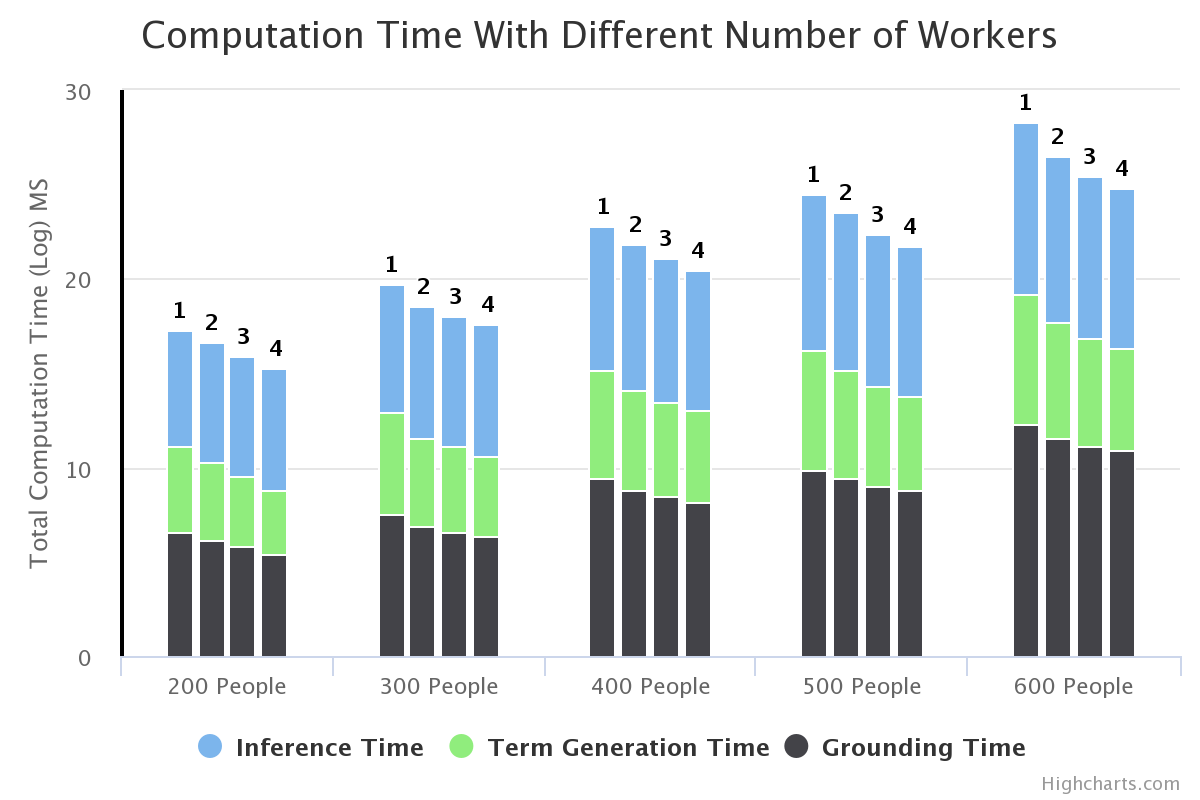
\includegraphics[width=\textwidth]{images/computationTimeTotal.png}
                    \caption{Broken Down Times}
                    \label{fig:distributed-results-computation-time-total}
                \end{subfigure}
                \begin{subfigure}{0.50\textwidth}
                    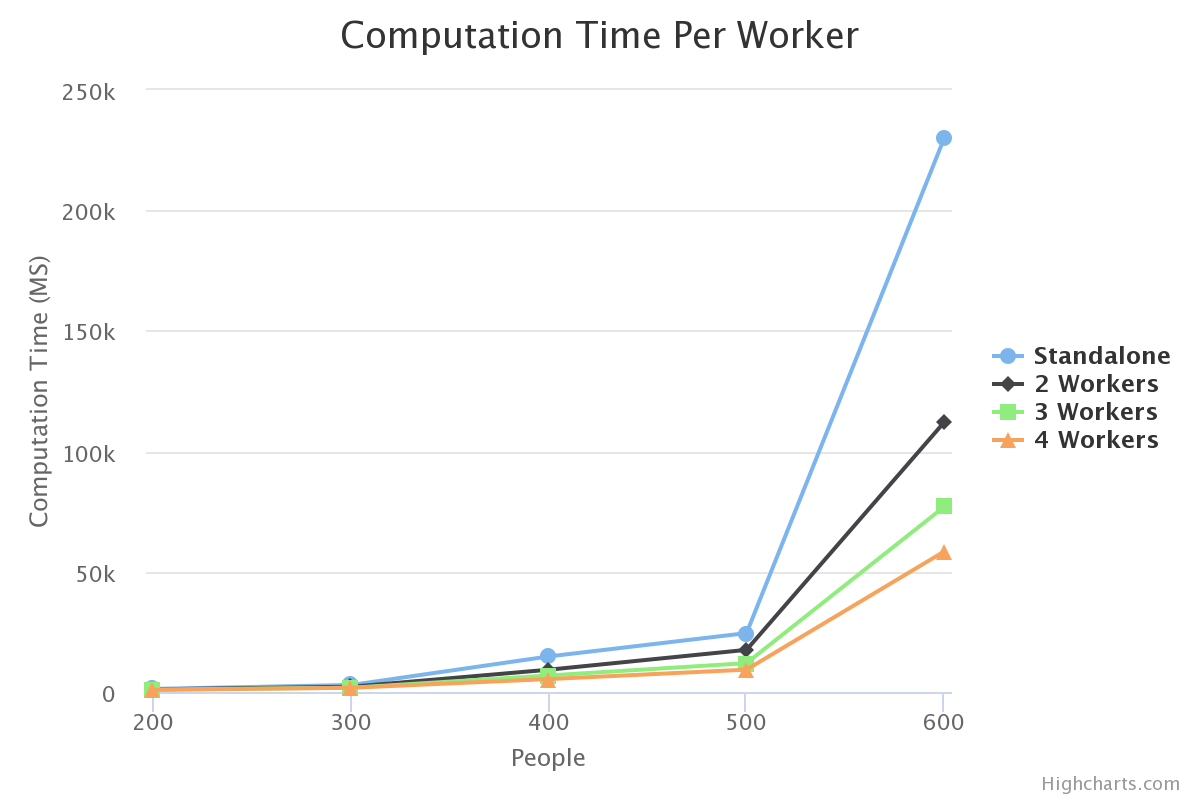
\includegraphics[width=\textwidth]{images/computationTimePerWorker.png}
                    \caption{Computation Time}
                    \label{fig:distributed-results-computation-time-worker}
                \end{subfigure}
                \caption{Runtimes for different number of workers.}
                \label{fig:distributed-results-runtimes}
            \end{figure}
            
            \begin{figure}
                \begin{subfigure}{0.50\textwidth}
                    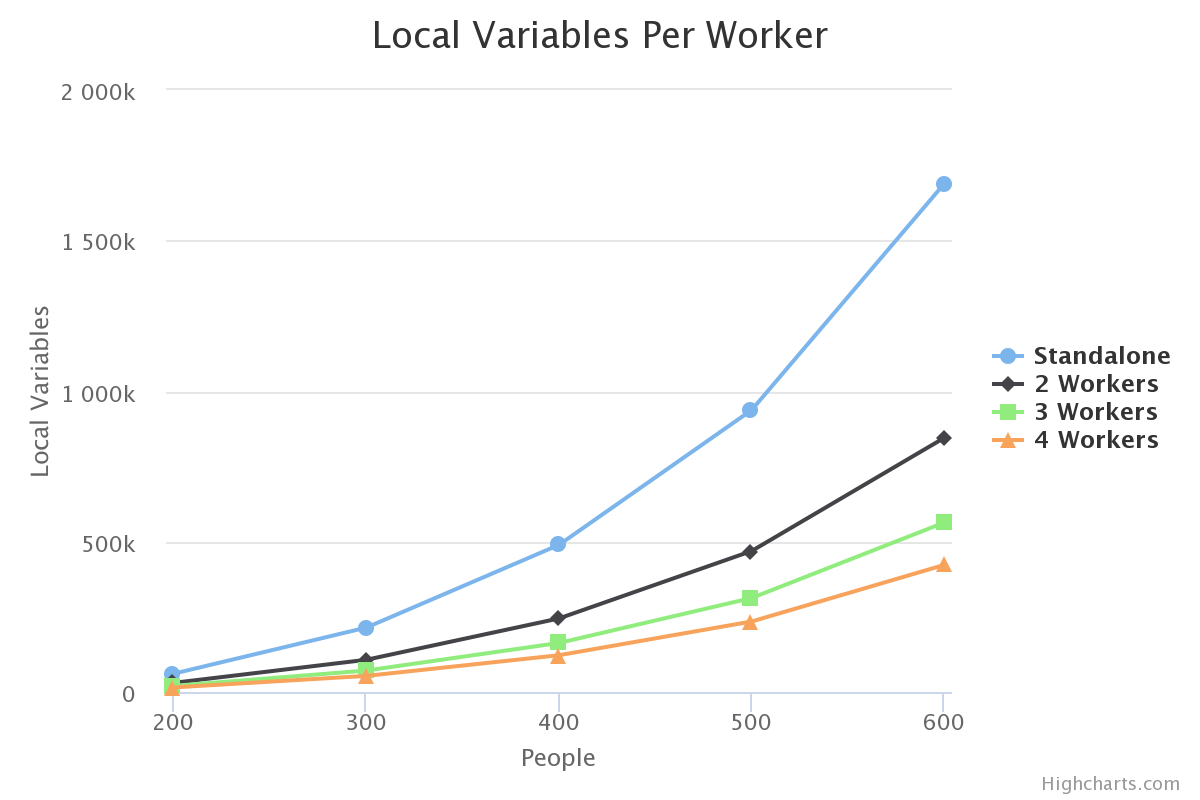
\includegraphics[width=\textwidth]{images/localVariablesPerWorker.png}
                    \caption{Local Variables}
                    \label{fig:distributed-results-local-variables}
                \end{subfigure}
                \begin{subfigure}{0.50\textwidth}
                    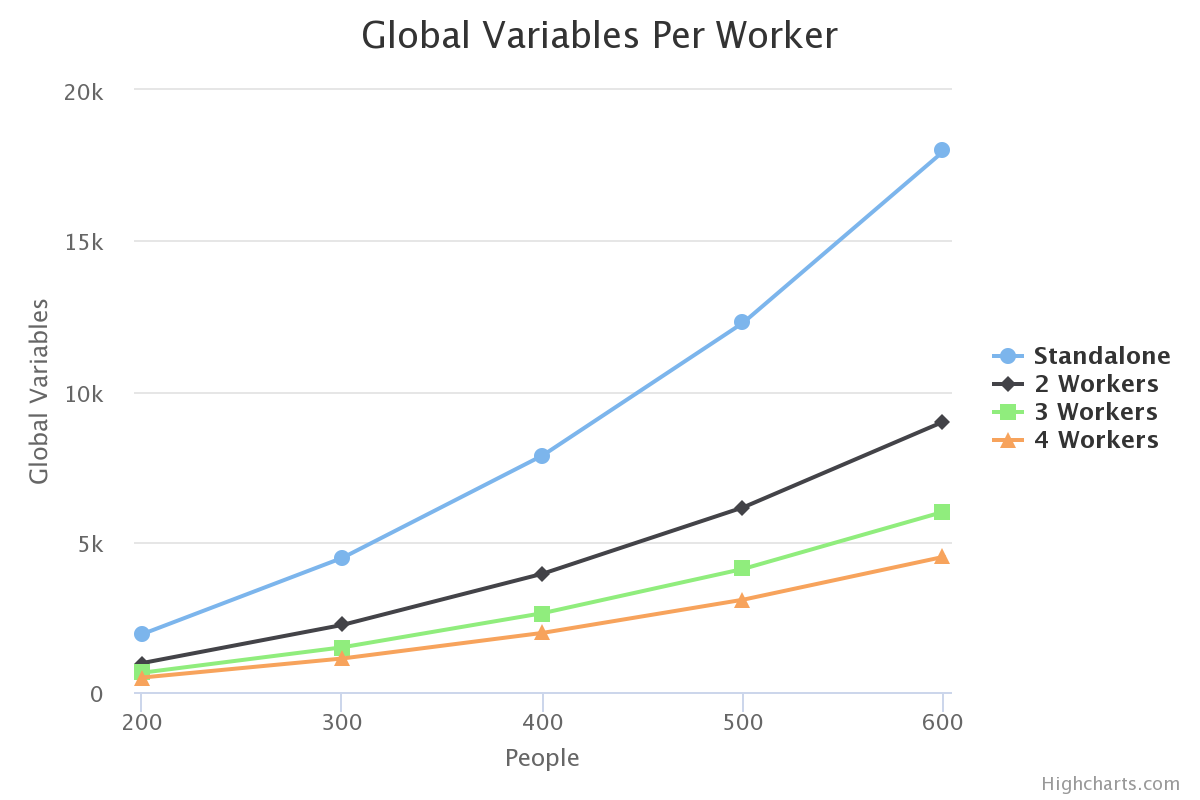
\includegraphics[width=\textwidth]{images/globalVariablesPerWorker.png}
                    \caption{Global Variables}
                    \label{fig:distributed-results-global-variables}
                \end{subfigure}
                \caption{The mean number of variables on a worker.}
                \label{fig:distributed-results-variables}
            \end{figure}
            
            \begin{figure}
                \centering
                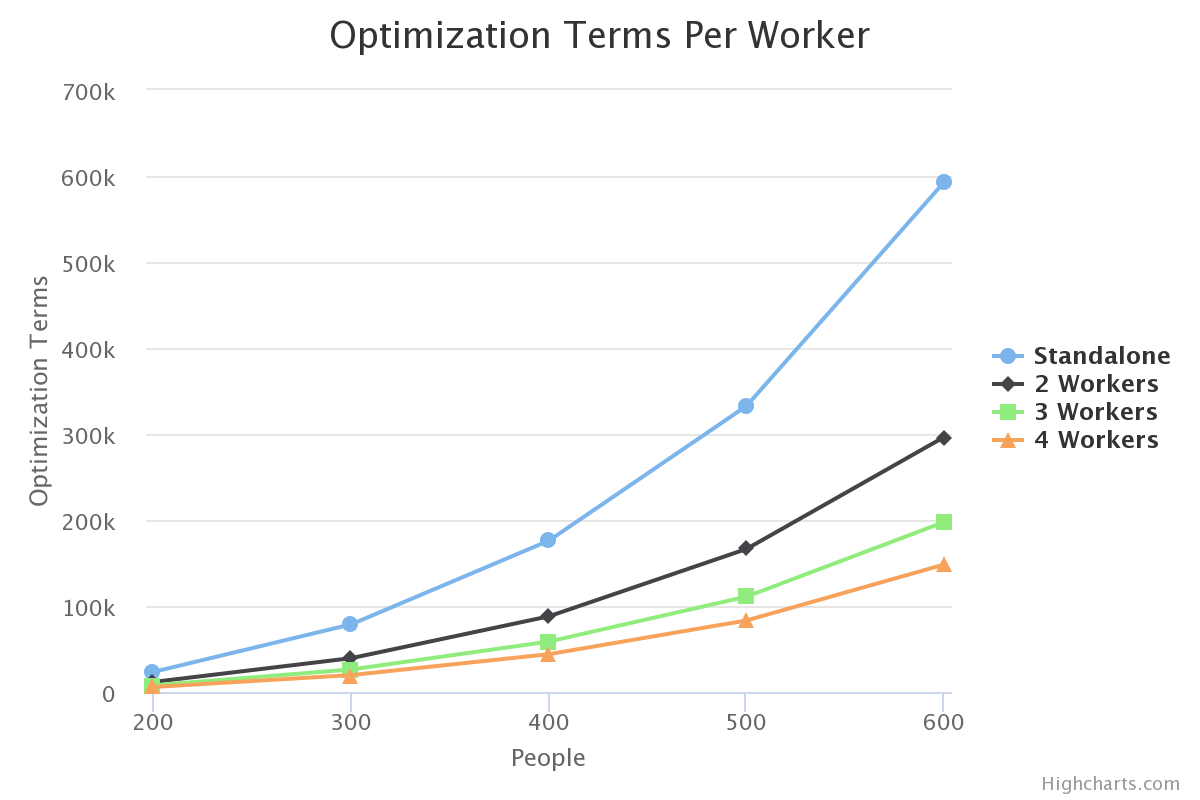
\includegraphics[width=0.80\textwidth]{images/optimizationTermsPerWorker.png}
                \caption{The mean number of optimization terms (ground rules) on a worker.}
                \label{fig:distributed-results-terms}
            \end{figure}
    
    \subsection{Bibliographic}
    
        \begin{table}
            \begin{center}
                \begin{tabular}{| c | c | c | c | c |}
                    \hline
                    & Auth Prec & Auth Recall & Pub Prec & Pub Recall \\
                    \hline
                    No Trans, BM4 & 0.7662 & 0.7888 & 0.9855 & 0.8718  \\
                    Trans, BM4    & \textbf{0.7913} & \textbf{0.8907} & 0.9855 & 0.8718  \\
                    No Trans, BM5 & 0.6186 & 0.0866 & 0.9855 & 0.8718  \\
                    Rule X, BM5    & 0.4042 & 0.1122 & 0.9855 & 0.8718  \\
                    \hline
                \end{tabular}
            \caption{Inference results with the CORA dataset}
            \label{tab:corauwash-prec-rec-results}
            \end{center}
        \end{table}        
    
        \begin{figure}
                \centering
                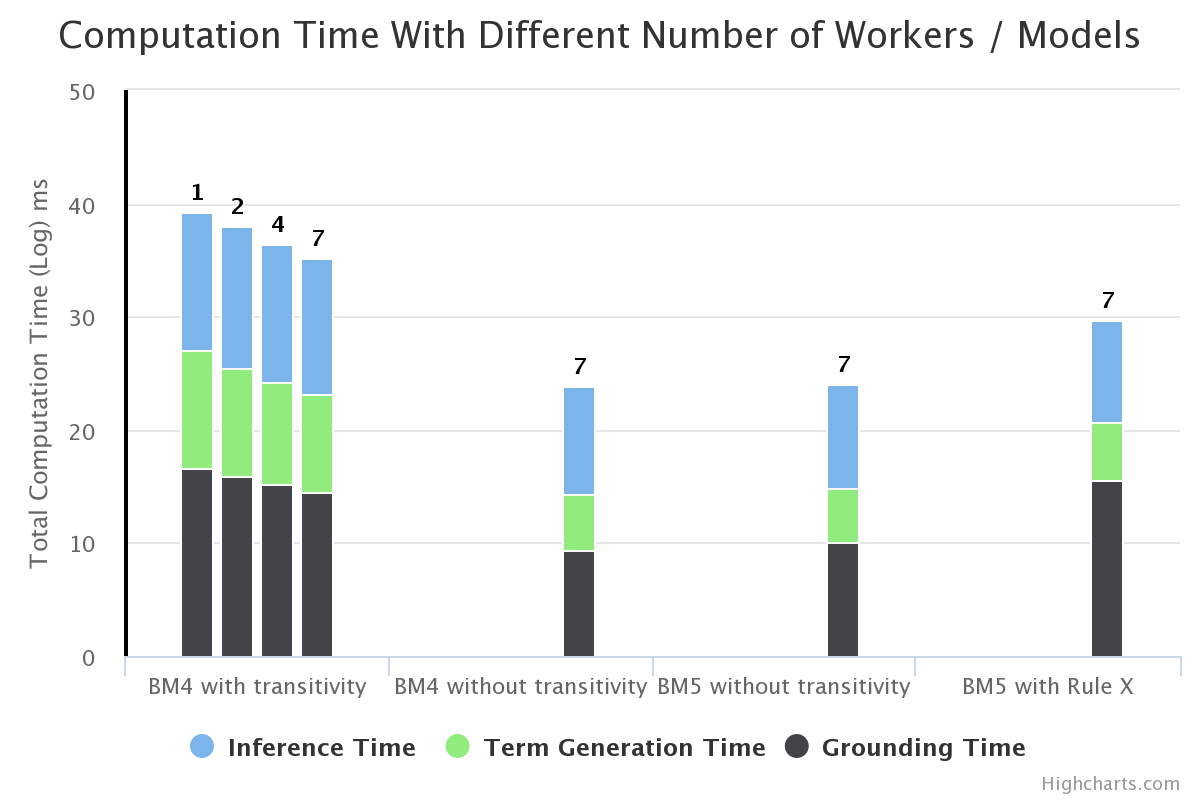
\includegraphics[width=0.80\textwidth]{images/CoraUWashResults-HighLevel.png}
                \caption{Comparison of execution times with variation in blocking methods, and transitivity rules.}
                \label{fig:corauwash-results}
            \end{figure}

        Results with the bibliographic data subset are shown in Figure \ref{fig:corauwash-results} and Table \ref{tab:corauwash-prec-rec-results}. To recap, BM4 is the blocking method that uses the first character of each token in the author mention, and BM5 is the two-level blocking method with $\eta$ = 0.1.
        
        We see from the table that transitivity certainly helps, proving the usefulness of the relational rule of transitivity, and justifying the cubic space complexity incurred. Since grounding takes a substantial amount of time, this translates to an increase in time complexity as well. As we see in Figure \ref{fig:corauwash-results} in the `BM4 with transitivity' category, a distributed implementation helps us deal with this by distributing the grounding across nodes, leading to improved grounding and overall execution times. 
        
        The BM4 with transitivity PSL model has 15.2 million ground rules. While a single node took 277 minutes to ground, grounding took place in 34 minutes, with seven nodes. 
        
        The hierarchical blocking method BM5 performs poorly. It buys us no precision, recall, nor even improved grounding times when coupled with rule X. However, this is expected since it will need a strong non-blocking rule that will propagate transitivity across the second level of blocks. It is a matter of surprise, however, that the recall after inference is poorer than what recall is offered at the level of blocking.
        

\section{Related Work}
    
    \subsection{Entity resolution}
        
        Statistical relational techniques have been previously applied to entity resolution.
        Notably, \cite{singla2006entity} address Entity Resolution using Markov Logic Networks.
        \cite{bhattacharya:thesis06} predates PSL, contains important work about formulating ER as a collective inference problem.
        It compares several similarity and neighbourhood similarity metrics, and introduces a relational clustering algorithm.
        For a more recent treatment, albeit within the context of knowledge graph ER, \cite{pujara:starai16} describes common modeling patterns and rules.
        
        \cite{kopcke2010frameworks} provide a nice overview of several entity resolution solutions.
        We use the same bibliographic datasets that they use enabling a comparison with their metrics.
        
        Distributed scaling has been successfully implemented in the past in \cite{pujara:thesis16} for knowledge graph identification (KGI), where a knowledge graph was partitioned across multiple machines.
        In the domain of ER, just as in the domain of KGI, the challenge lies in partitioning data without losing relationships in the graphical model.
        
    \subsection{Parallelizing Entity Resolution}
        
        There are several papers that specifically talk about distributing or parallelizing Entity Resolution problems.
        \cite{benjelloun2007d} and \cite{kawai2006p} presents a family of algorithms for distributing/parallelizing the ER workload across multiple processors.
        This is a family of algorithms because they treat the matching and record merging functions (as well as the distributing functions) as black boxes, where any relevant function of choice can be substituted.
        \cite{efthymiou2017parallel} introduces algorithms for Meta-blocking that use the Map Reduce framework.
        Meta-blocking is used to clean the overlapping blocks from unnecessary comparisons.
        \cite{dal2011fast}'s MD-approach combines an efficient blocking method with a robust data parallel programming model for a salable deduplication solution.
        \cite{malhotra2014graph} compare two distribution approaches that they call bucket-centric and record-centric with a focus on load balancing.
        \cite{kirsten2010data} propose different strategies to partition the input data and generate multiple match tasks that can be independently executed.
        \cite{kim2007parallel} study scenarios where the collections being compared/merged are clean, only one is clean, and both are dirty to exploit interplay between match and merge to achieve parallelization.
        \cite{rastogi2011large} propose a principled framework to scale any generic entity matching algorithm by running multiple instances of the EM algorithm on small neighborhoods of the data and passing messages across neighborhoods to construct a global solution.


\section{Discussion}
    Entity Resolution is a large problem that can quickly become unmanageable. A standard ER solution will grow to the order of the number of entities squared. In the collective inference setting, the addition of a transitivity rule will cause the problem to grow to the order of the number of entities cubed. To combat this growth, we have shown that blocking and distributing the optimization problem can be utilized to reduce the memory burden on a single machine and solve problems more quickly.
    
    We use a greedy selection of blocks (based on the size of elements in a block) to assign to nodes. In cases where the workers used are heterogeneous (as in our case with the bibliography ER experiments) there is room for improvement by assigning bigger blocks to more powerful machines. In all cases, we saw that the bottleneck was the grounding time on the least powerful server. 
    
    We also saw that there is merit in tightly coupling the blocking criterion with the distribution scheme, especially when the transitivity rule is used. Since the complexity of grounding is effectively cubic in the size of the block when using transitivity, smaller blocks can significantly reduce the total execution time. We noticed that the blocks were unevenly sized under the BM4 method. We hypothesize that a two step inference approach where the first step resolves the easier to resolve mentions to their entities followed by a round of inference on these `lifted' resolved entities may be a viable approach to solving the problem, and will be explored in future work. \cite{wick2009entity} have addressed this problem in the past.
    
    Overall, we successfully implemented a distributed implementation of PSL leveraging blocking for partitioning the data, making problems that hitherto did not fit on a single machine approachable, and the results also show a significant improvement in inference time, as grounding time reduces linearly with the number of machines added.

\appendix
\appendixpage

\section{Additional Diagrams}
    \label{appendix:additional-diagrams}

    \begin{figure}[H]
        \centering
        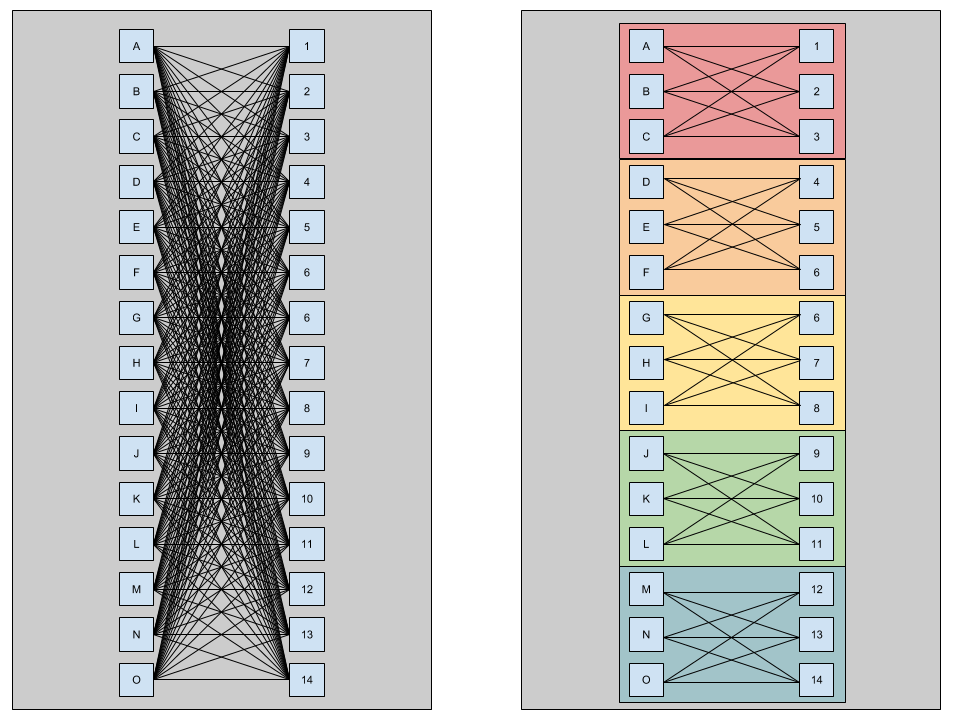
\includegraphics[width=\textwidth]{images/Blocking.png}
        \caption{Blocking reduces the number of comparisons from 196 on the left to 45 on the right.}
        \label{fig:blocking}
    \end{figure}

    \begin{figure}[H]
        \centering
        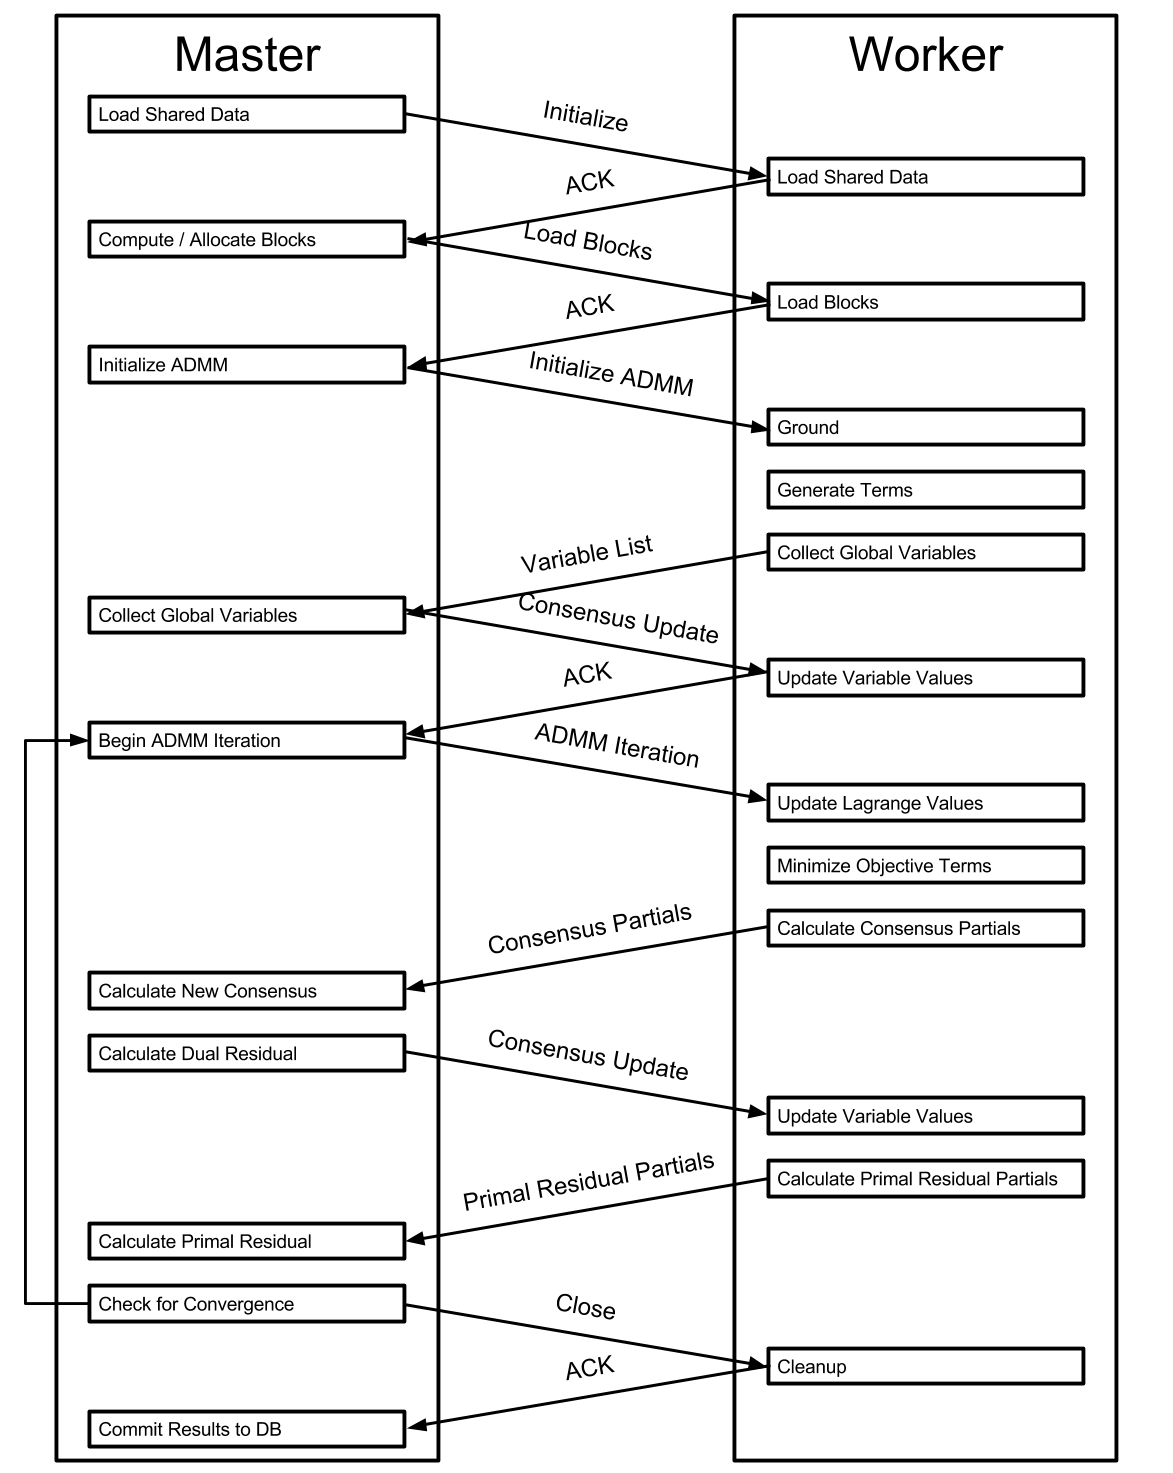
\includegraphics[width=\textwidth]{images/Distributed_ADMM_Workflow.png}
        \caption{The control flow between the master and worker nodes in the distributed ADMM implementation.}
        \label{fig:distributed-admm-workflow}
    \end{figure}

    \begin{figure}[H]
        \centering
        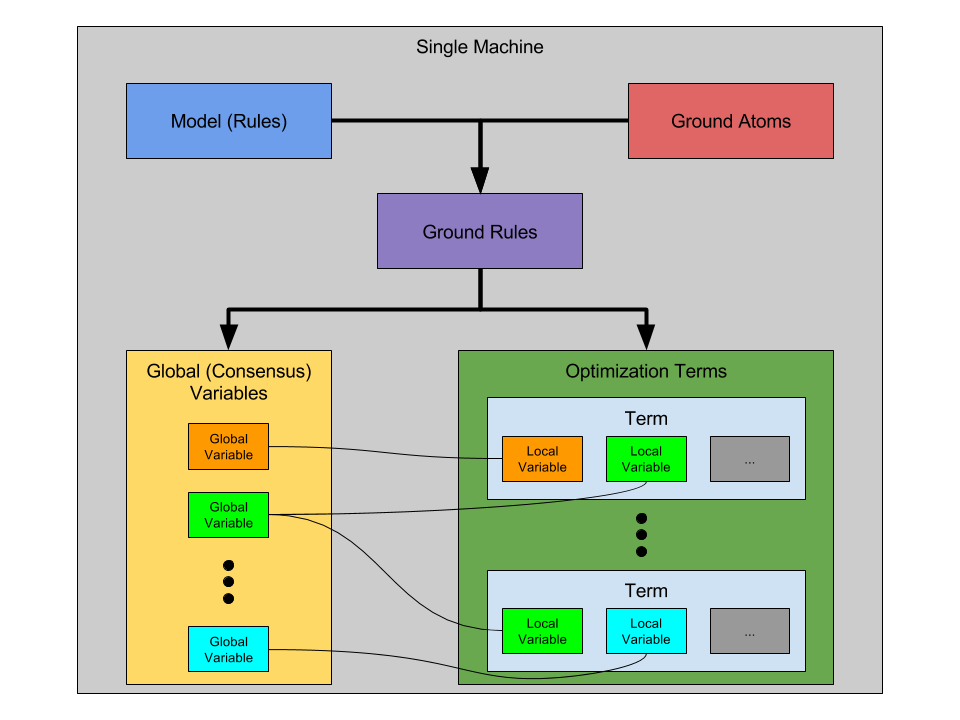
\includegraphics[width=\textwidth]{images/ADMM_Single_Machine.png}
        \caption{The location of critical pieces of data in our standalone ADMM implementation.}
        \label{fig:standalone-admm-data}
    \end{figure}

    \begin{figure}[H]
        \centering
        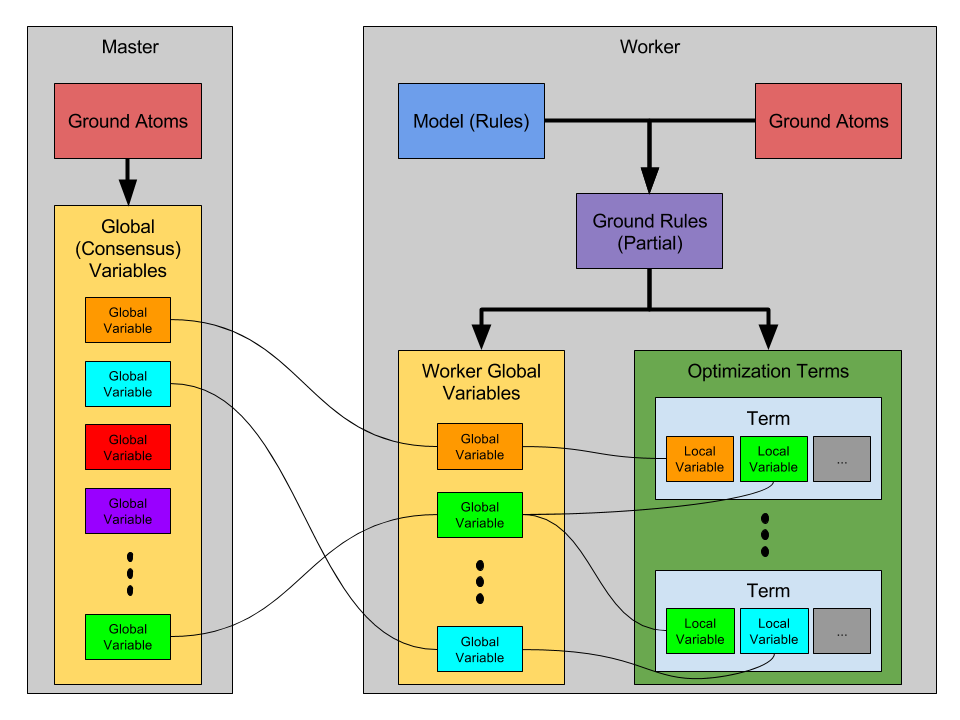
\includegraphics[width=\textwidth]{images/ADMM_Distributed.png}
        \caption{The location of critical pieces of data in our distributed ADMM implementation.}
        \label{fig:distributed-admm-data}
    \end{figure}
    
\section{Full Results}
   \label{appendix:full-results}

    Table \ref{tab:results-full-runtime} shows full runtime results on synthetic data.
    Table \ref{tab:results-full-variables} shows full term and variable results on synthetic data.

    \begin{table}[H]
        \small
        \begin{center}
            \begin{tabular}{| c | c | c | c | c | c | c |}
                \hline
                    People & Blocks & Workers & Grounding (ms) & Term Generation (ms) & Inference (ms) & Computation (ms) \\
                \hline
                    200 & 10 & 1 & 1783 & 182 & 1023 & 2988 \\
                    200 & 20 & 1 & 733 & 95 & 449 & 1277 \\
                    200 & 30 & 1 & 473 & 47 & 276 & 796 \\
                    300 & 10 & 1 & 5928 & 444 & 3769 & 10141 \\
                    300 & 20 & 1 & 1815 & 218 & 895 & 2928 \\
                    300 & 30 & 1 & 1029 & 121 & 495 & 1645 \\
                    400 & 10 & 1 & 21983 & 1107 & 8214 & 31304 \\
                    400 & 20 & 1 & 12288 & 301 & 2196 & 14785 \\
                    400 & 30 & 1 & 8324 & 229 & 906 & 9459 \\
                    500 & 10 & 1 & 66635 & 2111 & 18570 & 87316 \\
                    500 & 20 & 1 & 19828 & 547 & 4080 & 24455 \\
                    500 & 30 & 1 & 14391 & 289 & 1895 & 16575 \\
                    600 & 10 & 1 & 493776 & 4112 & 41014 & 538902 \\
                    600 & 20 & 1 & 219647 & 944 & 9287 & 229878 \\
                    600 & 30 & 1 & 154071 & 448 & 3073 & 157592 \\
                    200 & 10 & 2 & 928 & 122 & 1445 & 2495 \\
                    200 & 20 & 2 & 465 & 64 & 587 & 1116 \\
                    200 & 30 & 2 & 246 & 38 & 502 & 786 \\
                    300 & 10 & 2 & 2572 & 288 & 3694 & 6554 \\
                    300 & 20 & 2 & 976 & 106 & 1094 & 2176 \\
                    300 & 30 & 2 & 576 & 74 & 740 & 1390 \\
                    400 & 10 & 2 & 11733 & 497 & 8793 & 21023 \\
                    400 & 20 & 2 & 6771 & 190 & 2307 & 9268 \\
                    400 & 30 & 2 & 5892 & 111 & 1271 & 7274 \\
                    500 & 10 & 2 & 22534 & 1008 & 19127 & 42669 \\
                    500 & 20 & 2 & 12909 & 300 & 4298 & 17507 \\
                    500 & 30 & 2 & 10078 & 149 & 2335 & 12562 \\
                    600 & 10 & 2 & 229961 & 1851 & 27328 & 259140 \\
                    600 & 20 & 2 & 104648 & 471 & 6867 & 111986 \\
                    600 & 30 & 2 & 73800 & 262 & 3560 & 77622 \\
                    200 & 10 & 3 & 726 & 97 & 1278 & 2101 \\
                    200 & 20 & 3 & 342 & 39 & 604 & 985 \\
                    200 & 30 & 3 & 191 & 23 & 474 & 688 \\
                    300 & 10 & 3 & 1921 & 187 & 2725 & 4833 \\
                    300 & 20 & 3 & 713 & 92 & 971 & 1776 \\
                    300 & 30 & 3 & 398 & 52 & 720 & 1170 \\
                    400 & 10 & 3 & 7566 & 328 & 6886 & 14780 \\
                    400 & 20 & 3 & 4661 & 157 & 2061 & 6879 \\
                    400 & 30 & 3 & 4030 & 97 & 1107 & 5234 \\
                    500 & 10 & 3 & 14332 & 812 & 12526 & 27670 \\
                    500 & 20 & 3 & 8394 & 188 & 3413 & 11995 \\
                    500 & 30 & 3 & 6860 & 141 & 1738 & 8739 \\
                    600 & 10 & 3 & 137243 & 1108 & 19364 & 157715 \\
                    600 & 20 & 3 & 71582 & 304 & 4998 & 76884 \\
                    600 & 30 & 3 & 48313 & 170 & 2556 & 51039 \\
                    200 & 10 & 4 & 567 & 76 & 1527 & 2170 \\
                    200 & 20 & 4 & 226 & 30 & 623 & 879 \\
                    200 & 30 & 4 & 156 & 31 & 458 & 645 \\
                    300 & 10 & 4 & 1452 & 160 & 2817 & 4429 \\
                    300 & 20 & 4 & 569 & 72 & 1125 & 1766 \\
                    300 & 30 & 4 & 338 & 36 & 702 & 1076 \\
                    400 & 10 & 4 & 5932 & 285 & 10056 & 16273 \\
                    400 & 20 & 4 & 3531 & 126 & 1717 & 5374 \\
                    400 & 30 & 4 & 3040 & 73 & 1138 & 4251 \\
                    500 & 10 & 4 & 11393 & 526 & 18595 & 30514 \\
                    500 & 20 & 4 & 6351 & 155 & 2778 & 9284 \\
                    500 & 30 & 4 & 5240 & 116 & 1901 & 7257 \\
                    600 & 10 & 4 & 102056 & 1144 & 28093 & 131293 \\
                    600 & 20 & 4 & 53408 & 234 & 4685 & 58327 \\
                    600 & 30 & 4 & 37323 & 150 & 2534 & 40007 \\
                \hline
            \end{tabular}
            \caption{Full runtime results.}
            \label{tab:results-full-runtime}
        \end{center}
    \end{table}


    \begin{table}[H]
        \tiny
        \centering
        \begin{center}
            \begin{tabular}{| c | c | c | c | c | c | c | c | c | c | c | c | c | c | c |}
                \hline
                    People & Nodes & Blocks & \thead{\tiny Node 1 \\ \tiny Terms} & \thead{\tiny Node 1 \\ \tiny Local} & \thead{\tiny Node 1 \\ \tiny Global} & \thead{\tiny Node 2 \\ \tiny Terms} & \thead{\tiny Node 2 \\ \tiny Local} & \thead{\tiny Node 2 \\ \tiny Global} & \thead{\tiny Node 3 \\ \tiny Terms} & \thead{\tiny Node 3 \\ \tiny Local} & \thead{\tiny Node 3 \\ \tiny Global} & \thead{\tiny Node 4 \\ \tiny Terms} & \thead{\tiny Node 4 \\ \tiny Local} & \thead{\tiny Node 4 \\ \tiny Global} \\
                \hline
                    200 & 1 & 10 & 86191 & 239089 & 3906 & - & - & - & - & - & - & - & - & - \\
                    200 & 1 & 20 & 23516 & 60968 & 1920 & - & - & - & - & - & - & - & - & - \\
                    200 & 1 & 30 & 12916 & 32134 & 1326 & - & - & - & - & - & - & - & - & - \\
                    300 & 1 & 10 & 290256 & 826202 & 8930 & - & - & - & - & - & - & - & - & - \\
                    300 & 1 & 20 & 78764 & 214046 & 4458 & - & - & - & - & - & - & - & - & - \\
                    300 & 1 & 30 & 36382 & 94594 & 2916 & - & - & - & - & - & - & - & - & - \\
                    400 & 1 & 10 & 676125 & 1949021 & 15908 & - & - & - & - & - & - & - & - & - \\
                    400 & 1 & 20 & 176031 & 488853 & 7866 & - & - & - & - & - & - & - & - & - \\
                    400 & 1 & 30 & 85925 & 231279 & 5314 & - & - & - & - & - & - & - & - & - \\
                    500 & 1 & 10 & 1306446 & 3795226 & 24880 & - & - & - & - & - & - & - & - & - \\
                    500 & 1 & 20 & 332686 & 936826 & 12276 & - & - & - & - & - & - & - & - & - \\
                    500 & 1 & 30 & 158484 & 434366 & 8234 & - & - & - & - & - & - & - & - & - \\
                    600 & 1 & 10 & 2305962 & 6737342 & 36200 & - & - & - & - & - & - & - & - & - \\
                    600 & 1 & 20 & 592873 & 1688919 & 17978 & - & - & - & - & - & - & - & - & - \\
                    600 & 1 & 30 & 265055 & 736187 & 11820 & - & - & - & - & - & - & - & - & - \\
                    200 & 2 & 10 & 50097 & 139511 & 2162 & 36094 & 99578 & 1744 & - & - & - & - & - & - \\
                    200 & 2 & 20 & 10843 & 27959 & 916 & 12673 & 33009 & 1004 & - & - & - & - & - & - \\
                    200 & 2 & 30 & 5607 & 13647 & 636 & 7309 & 18487 & 690 & - & - & - & - & - & - \\
                    300 & 2 & 10 & 150425 & 429693 & 4324 & 139831 & 396509 & 4606 & - & - & - & - & - & - \\
                    300 & 2 & 20 & 39962 & 108636 & 2254 & 38802 & 105410 & 2204 & - & - & - & - & - & - \\
                    300 & 2 & 30 & 15027 & 38427 & 1332 & 21355 & 56167 & 1584 & - & - & - & - & - & - \\
                    400 & 2 & 10 & 354004 & 1023308 & 7756 & 322121 & 925713 & 8152 & - & - & - & - & - & - \\
                    400 & 2 & 20 & 85240 & 236410 & 3870 & 90791 & 252443 & 3996 & - & - & - & - & - & - \\
                    400 & 2 & 30 & 42399 & 113797 & 2686 & 43526 & 117482 & 2628 & - & - & - & - & - & - \\
                    500 & 2 & 10 & 864840 & 2518642 & 15214 & 441606 & 1276584 & 9666 & - & - & - & - & - & - \\
                    500 & 2 & 20 & 160173 & 450775 & 5962 & 172513 & 486051 & 6314 & - & - & - & - & - & - \\
                    500 & 2 & 30 & 77323 & 212085 & 3986 & 81161 & 222281 & 4248 & - & - & - & - & - & - \\
                    600 & 2 & 10 & 1267273 & 3711333 & 18140 & 1038689 & 3026009 & 18060 & - & - & - & - & - & - \\
                    600 & 2 & 20 & 290480 & 826592 & 8988 & 302393 & 862327 & 8990 & - & - & - & - & - & - \\
                    600 & 2 & 30 & 141302 & 392924 & 6210 & 123753 & 343263 & 5610 & - & - & - & - & - & - \\
                    200 & 3 & 10 & 31036 & 85784 & 1468 & 22111 & 60983 & 1072 & 33044 & 92322 & 1366 & - & - & - \\
                    200 & 3 & 20 & 6802 & 17410 & 600 & 7407 & 19077 & 630 & 9307 & 24481 & 690 & - & - & - \\
                    200 & 3 & 30 & 2849 & 6779 & 354 & 4494 & 11144 & 470 & 5573 & 14211 & 502 & - & - & - \\
                    300 & 3 & 10 & 84783 & 240969 & 2682 & 100365 & 285125 & 3200 & 105108 & 300108 & 3048 & - & - & - \\
                    300 & 3 & 20 & 22145 & 59869 & 1316 & 24284 & 65852 & 1404 & 32335 & 88325 & 1738 & - & - & - \\
                    300 & 3 & 30 & 14647 & 38381 & 1114 & 9152 & 23354 & 822 & 12583 & 32859 & 980 & - & - & - \\
                    400 & 3 & 10 & 235473 & 679703 & 5354 & 213699 & 616451 & 4940 & 226953 & 652867 & 5614 & - & - & - \\
                    400 & 3 & 20 & 51792 & 143012 & 2480 & 48455 & 133739 & 2328 & 75784 & 212102 & 3058 & - & - & - \\
                    400 & 3 & 30 & 31727 & 85797 & 1882 & 22800 & 60962 & 1490 & 31398 & 84520 & 1942 & - & - & - \\
                    500 & 3 & 10 & 469009 & 1364551 & 8514 & 417329 & 1213207 & 7778 & 420108 & 1217468 & 8588 & - & - & - \\
                    500 & 3 & 20 & 96085 & 269471 & 3766 & 136214 & 385836 & 4570 & 100387 & 281519 & 3940 & - & - & - \\
                    500 & 3 & 30 & 57221 & 157459 & 2846 & 47659 & 130301 & 2542 & 53604 & 146606 & 2846 & - & - & - \\
                    600 & 3 & 10 & 810841 & 2371249 & 12288 & 718727 & 2094819 & 12304 & 776394 & 2271274 & 11608 & - & - & - \\
                    600 & 3 & 20 & 221175 & 630883 & 6544 & 200276 & 571484 & 5880 & 171422 & 486552 & 5554 & - & - & - \\
                    600 & 3 & 30 & 86401 & 240087 & 3830 & 76070 & 210504 & 3550 & 102584 & 285596 & 4440 & - & - & - \\
                    200 & 4 & 10 & 20412 & 56218 & 1006 & 19864 & 55186 & 882 & 16230 & 44392 & 862 & 29685 & 83293 & 1156 \\
                    200 & 4 & 20 & 4408 & 11128 & 420 & 5458 & 14088 & 458 & 6536 & 17076 & 508 & 7114 & 18676 & 534 \\
                    200 & 4 & 30 & 2339 & 5549 & 294 & 1877 & 4433 & 240 & 4342 & 11090 & 388 & 4358 & 11062 & 404 \\
                    300 & 4 & 10 & 53933 & 153113 & 1740 & 100055 & 285373 & 2966 & 48706 & 137004 & 1826 & 87562 & 250712 & 2398 \\
                    300 & 4 & 20 & 22305 & 60813 & 1224 & 19856 & 53836 & 1148 & 20526 & 55870 & 1144 & 16077 & 43527 & 942 \\
                    300 & 4 & 30 & 10506 & 27640 & 778 & 7035 & 17991 & 624 & 10131 & 26569 & 766 & 8710 & 22394 & 748 \\
                    400 & 4 & 10 & 188903 & 546465 & 4054 & 124917 & 357465 & 3468 & 133905 & 385895 & 3170 & 228400 & 659196 & 5216 \\
                    400 & 4 & 20 & 50291 & 140279 & 2124 & 42403 & 117431 & 1960 & 38123 & 105415 & 1796 & 45214 & 125728 & 1986 \\
                    400 & 4 & 30 & 21182 & 57066 & 1300 & 19991 & 53767 & 1244 & 20243 & 54385 & 1274 & 24509 & 66061 & 1496 \\
                    500 & 4 & 10 & 371596 & 1082916 & 6392 & 271082 & 783902 & 5880 & 276186 & 802758 & 5172 & 387582 & 1125650 & 7436 \\
                    500 & 4 & 20 & 89757 & 253171 & 3226 & 80881 & 227619 & 3014 & 70454 & 197594 & 2760 & 91594 & 258442 & 3276 \\
                    500 & 4 & 30 & 43394 & 119482 & 2144 & 28816 & 77914 & 1710 & 42734 & 117492 & 2146 & 43540 & 119478 & 2234 \\
                    600 & 4 & 10 & 784824 & 2301896 & 10544 & 412348 & 1203408 & 6740 & 437548 & 1272216 & 8108 & 671242 & 1959822 & 10808 \\
                    600 & 4 & 20 & 129487 & 367757 & 4150 & 163772 & 467810 & 4710 & 143831 & 409163 & 4476 & 155783 & 444189 & 4642 \\
                    600 & 4 & 30 & 72565 & 202319 & 3082 & 50102 & 137778 & 2512 & 70466 & 196448 & 2994 & 71922 & 199642 & 3232 \\
                \hline
            \end{tabular}
            \caption{Full term and variables results.}
            \label{tab:results-full-variables}
        \end{center}
    \end{table}


\newpage

\bibliography{references} 
\bibliographystyle{apalike}

\end{document}
